\chapter{Architektur}
Nachdem wir unser Projektziel für uns gesetzt hatten, mussten wir überlegen, wie es sich realisieren lässt. Als erstes einigten wir uns darauf, dass wir einen Raspberry Pi für die externe Zugsteuerung benutzen. Dann mussten wir uns überlegen, wie wir den Zug mit dem Raspberry Pi kommunizieren lassen, damit die Geräte Information zwischen einander austauschen können. Bevor wir das allerdings entscheiden konnten, haben wir geschaut was der Zug und der Raspberry Pi machen müssen.\\
\\
Zuerst haben wir uns überlegt, was der Zug können muss, was vereinfacht gesagt lediglich das Transportieren von Fahrgästen von einem Bahnhof zu einem anderen Bahnhof ist. Daraus konnten wir ableiten, dass die Erkennung seiner aktuellen Position eine der wichtigsten Aufgaben des Zuges ist, denn wenn wir nicht wissen, wo der Zug ist, können wir ihm auch nicht sagen, wo er hinfahren soll. Des weiteren muss der Zug einstellen können, wie schnell er fährt, und Information übermitteln können. Damit hatten wir den ersten Entwurf der Funktionalität des Zuges bestimmt und konnten uns dem Raspberry Pi zuwenden. Dieser muss als eine externe Steuereinheit bestimmen, welchen Weg der Zug fahren soll. Dazu braucht er die Informationen über die Position des Zuges, an welchem Bahnhof Personen stehen und wohin diese gehen wollen. Des weiteren muss er dem Zug übermitteln können, wohin er als nächstes fahren soll. Mit unseren Überlegungen hatten wir schon automatisch unsere dritte Frage beantwortet. Denn der Zug muss dem Raspberry Pi seine aktuelle Position übermitteln und der Raspberry Pi muss dem Zug einen Befehl schicken, wohin und mit welcher Geschwindigkeit er als nächstes fahren soll. \\
\\
Nachdem wir unsere Fragen beantwortet hatten, wollten wir diese mit Hilfe eines Klassendiagramms konkretisieren (siehe Abbildung \ref{pic:ClassDiagram}). Im Nachfolgenden sind alle Klassen, die Thread in ihrem Namen haben, auch Threads. \textit{LocateThread} in der Train-Komponente des Klassendiagramms beschäftigt sich ausschließlich mit der Bestimmung der Position des Zuges. Zur Bestimmung der Position haben wir auf der Strecke RFID-Tags verteilt, die \textit{LocateThread} beim Überfahren lesen kann und die er weiter an \textit{TrainSpeakerThread} schickt. Dieser vergleicht nach dem Erhalten der Position diese mit der eingetragenen Position in \textit{Order}. Falls die Positionen sich unterscheiden, ist entweder etwas schiefgelaufen oder der Zug ist gerade erst angefahren und hat zum ersten mal seine Position bestimmt. In beiden Fällen wird die Geschwindigkeit des Zuges auf 0 gesetzt und er wartet somit auf weitere Befehle. Falls die Positionen gleich sind, wird die \textit{afterSpeed} Geschwindigkeit aus \textit{Order} genommen und dem \textit{TrainThread} übermittelt, welcher dann diese Geschwindigkeit setzt. Als letztes schickt \textit{TrainSpeakerThread} über eine Socket-Verbindung die Position des Zuges an den Raspberry Pi. Diese Nachricht kommt dann an \textit{PiListenerThread}, welcher diese in \textit{TrainStatus} abspeichert. Danach kann \textit{PiAlgorithm} die aktuelle Position des Zuges aus \textit{TrainStatus} auslesen und bestimmen, wohin der Zug als nächstes fahren soll(genaueres wird im Kapitel Algorithmus erklärt). Diesen Befehl schickt er an \textit{PiSpeakerThread}, welcher diesen weiter über die Socket-Verbindung schickt. Der Befehl wird von \textit{TrainListenerThread} erhalten, welcher den Befehl in \textit{Order} speichert. Zuletzt wird noch die \textit{beforeSpeed} Geschwindigkeit, die im Befehl enthalten ist, an den \textit{TrainThread} übermittelt, welcher dann die Geschwindigkeit des Zuges darauf setzt. Damit hätte man einen gesamten Durchlauf gemacht, welcher wieder von Neuem beginnt, wenn der Zug eine neue Position liest.  


\begin{figure}[H]	
\caption{Klassendiagramm}
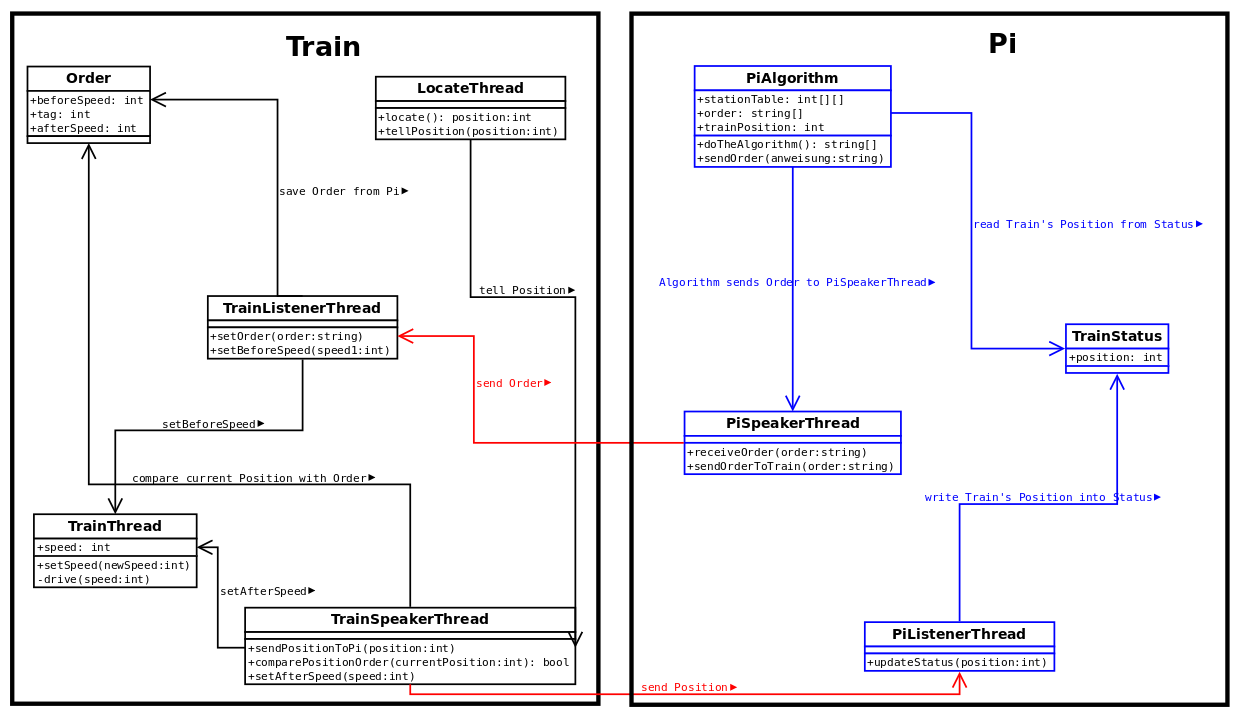
\includegraphics[width=2\textwidth, width=700pt, angle =90]{content/images/ClassDiagram.png}
\label{pic:ClassDiagram}
\end{figure}

\begin{figure}[H]	
\caption{Use Case Diagramm}
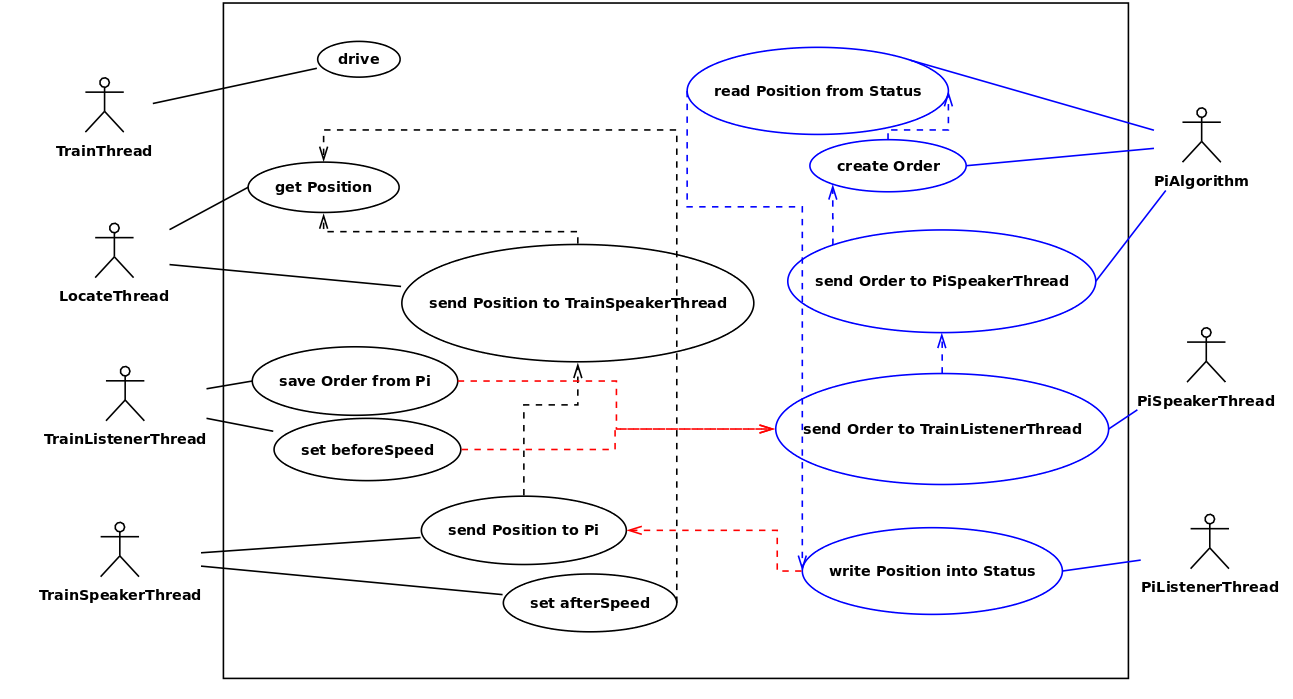
\includegraphics[width=2\textwidth, width=465pt]{content/images/UseCaseDia.png}
\label{pic:UseCaseDiagram}
\end{figure}

\begin{figure}[H]	
\caption{Beschreibung von ausgewählten Use Cases}
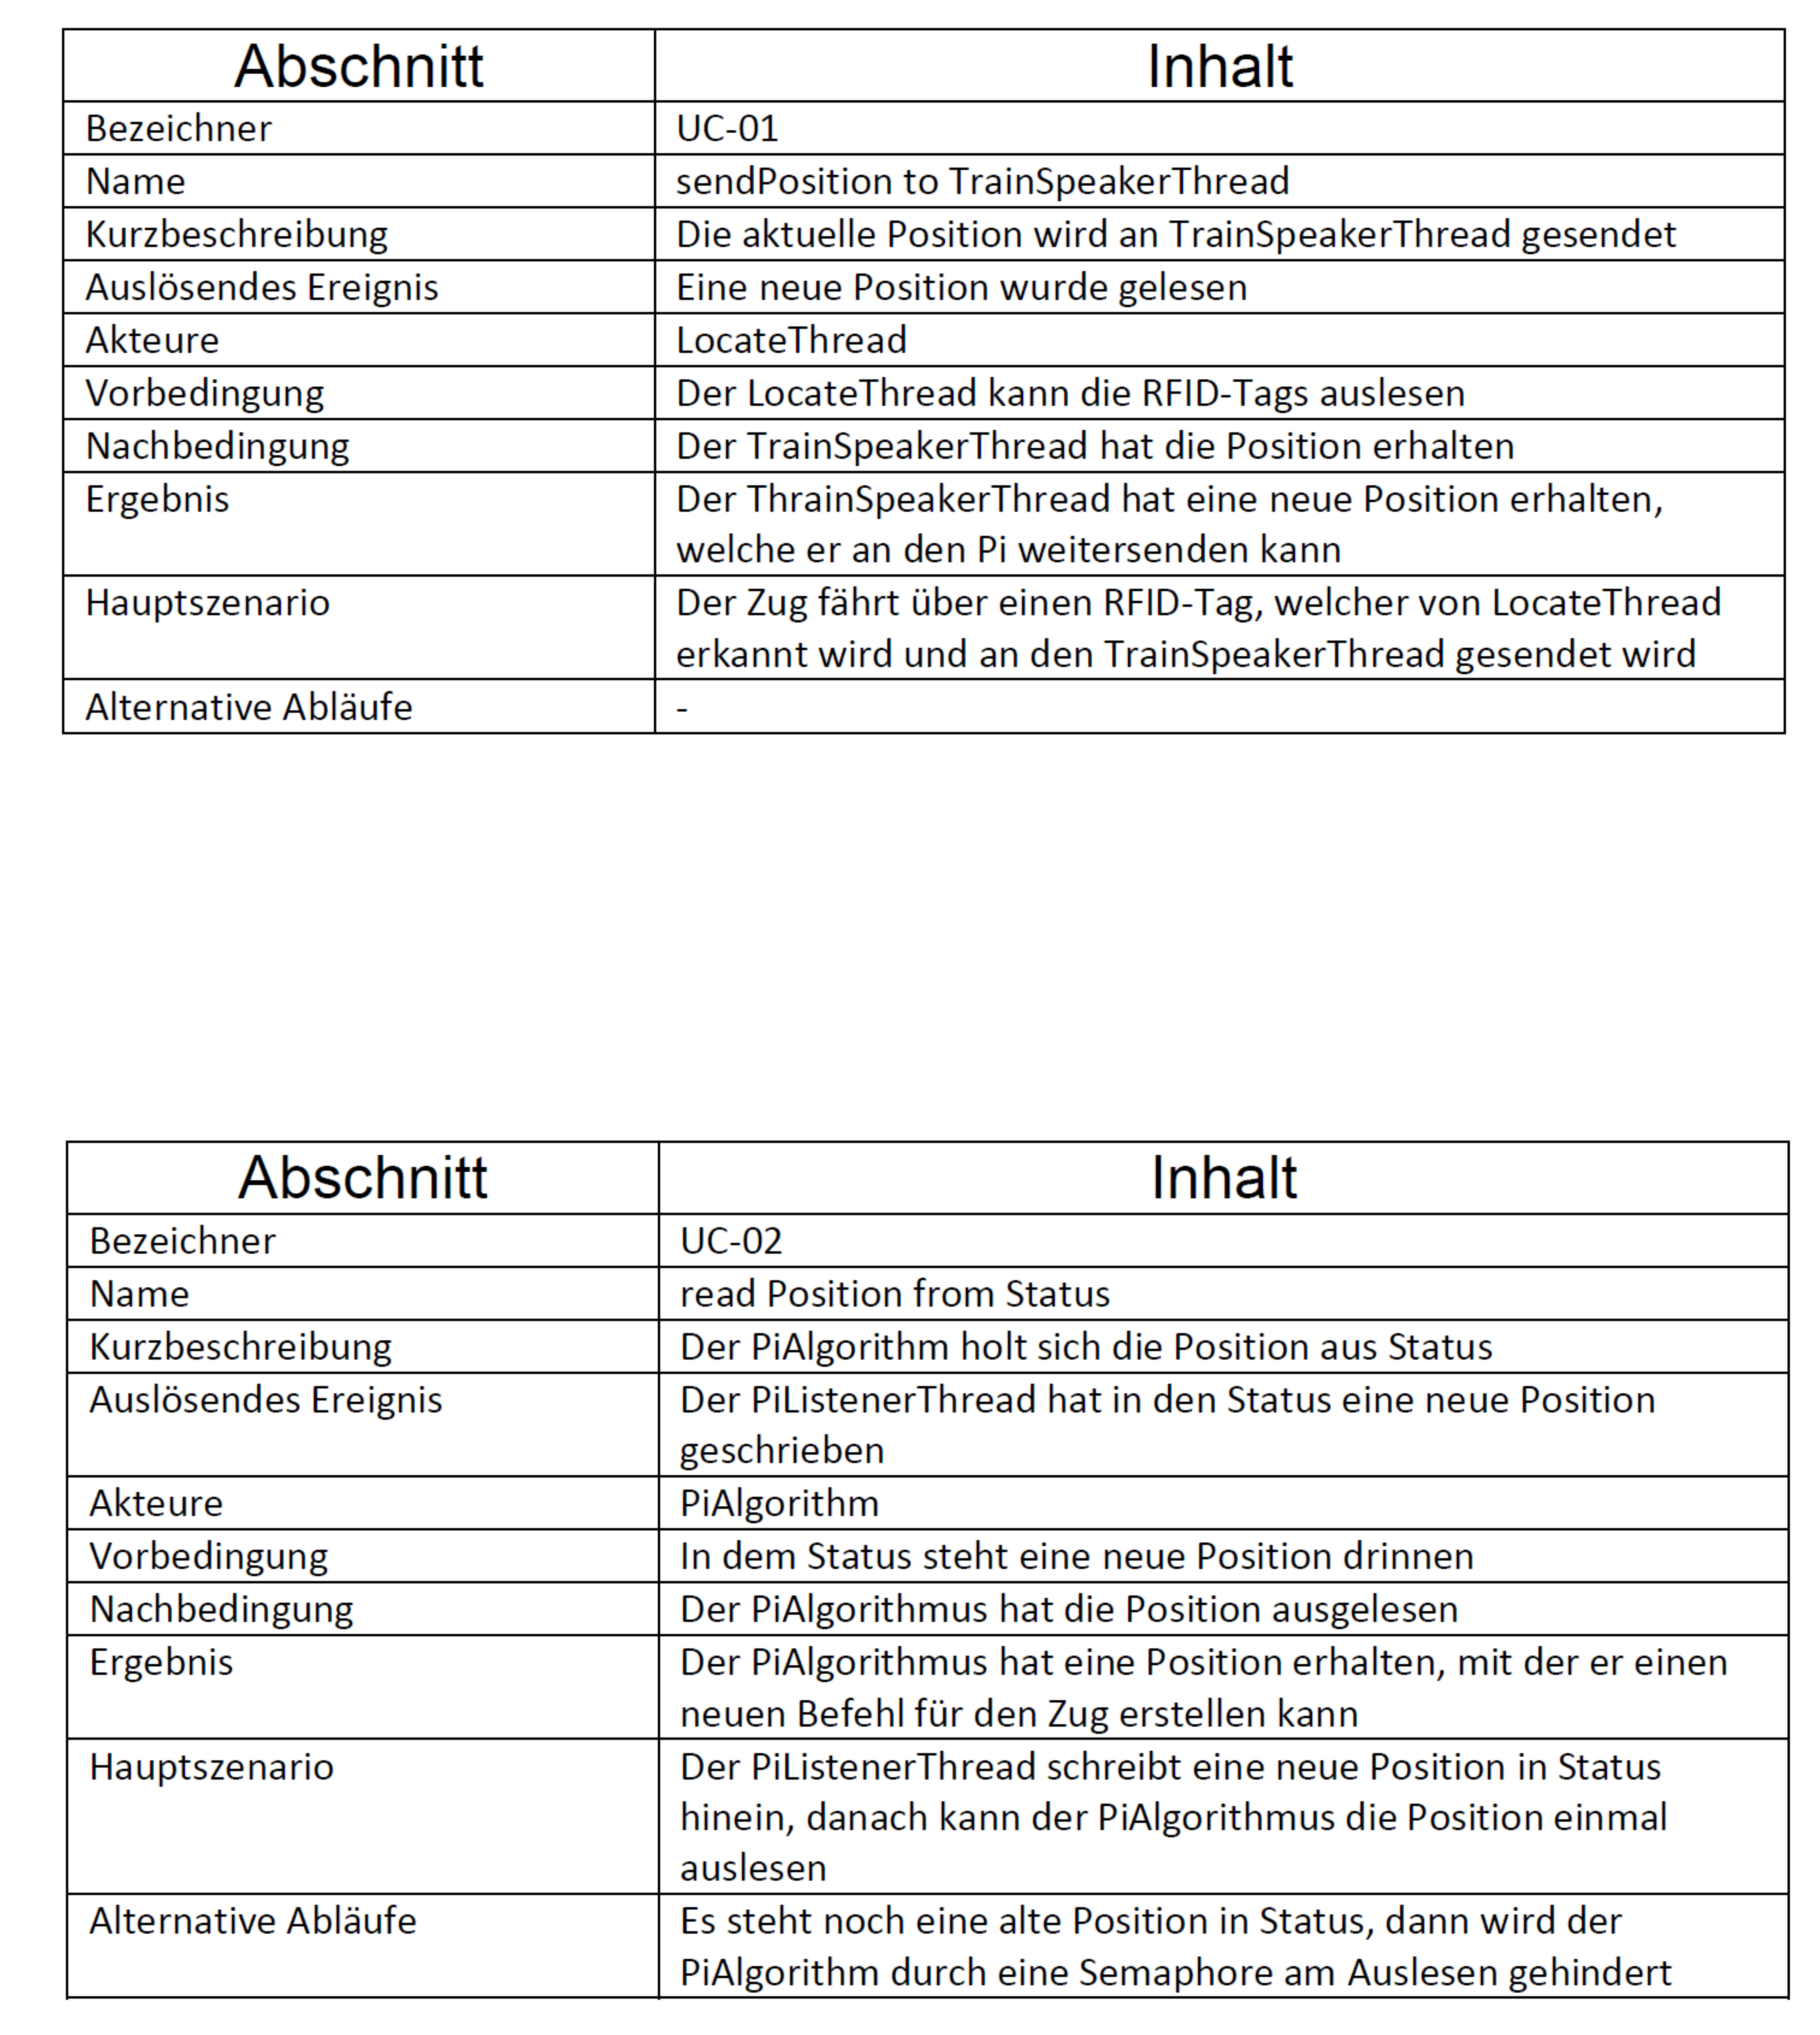
\includegraphics[width=2\textwidth, width=445pt]{content/images/UseCase1.png}
\label{pic:UseCase1}
\end{figure}
